\section{Topic 5. Numerical Methods for Initial Value Problems}
\subsection{Defining Initial Value Problems}
We can write the initial value problem,
\[
\begin{cases}
	y^{\prime}(t) = f(t, y(t)) \\
	y(0) = y_0
\end{cases}
\]
for $t \in [0, T]$ as
\[y(t) = y_0 + \int_0^t \underbrace{f(s, y(s))}_{y^{\prime}(s)} ds\]
using the Fundamental Theorem of Calculus. In many cases, we cannot obtain an explicit formula for  $y(t)$. Using numerical methods, $f$ can be approximated by a reasonably smooth function. 

We will choose a uniformly spaced step size $h = T / N$ to step forward on each $t_n = nh$ by solving a discrete set of algebraic equations for $y_n$ that approximates the value of $y(t_n)$. This discrete set of algebraic equations is called a \textbf{discretization}. One way to find a discretization is to approximate $y^{\prime}$ by a finite difference.
\[
\begin{cases}
	y^{\prime}(t) = f(t, y(t)) \\
	y(0) = y_0
\end{cases} \rightarrow \quad \begin{cases}
	\mathbf{D}_h (y(t_n)) = f(t_n, y_n) \\
	y_0 \text{ is given}
\end{cases}
\]

\begin{defn}[Explicit Discretization]
	A discretization is \textbf{explicit} if $y_{n+1}$ can be solved for explicitly. Otherwise, it is called \textbf{implicit}.
\end{defn}

\begin{rmk}
	Implicit methods require root finding at each time step $t_n$ to solve for $y_{n+1}$. This makes them costly computationally, but they generally have better stability properties.
\end{rmk}

\begin{defn}[$k$-Step]
	A discretization is called \textbf{$k$-step} if it requires knowing $k$ previous  steps $y_n, \cdots, y_{n-k+1}$ to compute $y_{n+1}$.
\end{defn}

\subsection{Methods based on Numerical Differentiation}

\begin{ex}{Explicit and Implicit Discretization}{label}
	We have seen the following approximations for $\mathbf{D}_h(y(t_n))$:
	\begin{enumerate}
	\item The \textbf{forward difference} formula is a $1$ step explicit method
	\[y_{n+1}=y_n+h f\left(t_n, y_n\right)\]
	\item The \textbf{backward difference} formula is $2$ step implicit method
	\[y_{n+1}=y_n+h f\left(t_{n+1}, y_{n+1}\right)\]
	\item The \textbf{central difference} formula is $2$ step explicit method
	\[y_{n+1}=y_{n-1}+2 h f\left(t_n, y_n\right)\]
	\end{enumerate}
\end{ex}

\begin{ex}{Studying Population Dynamics}{label}
	Let $N(t)$ be the number of individuals in a given population at time $t$. Consider the differential equation,
	\[\frac{dN}{dt} = \frac{r}{k}(K - N(t)) \cdot N(t)\]
	for a positive \textbf{rate} $r$ and a \textbf{carrying capacity} $k$ of the environment. Consider the initial value problem,
	\[
	\begin{cases}
		y^{\prime} = \frac{1}{5} (10 - y) y &\\
		y_0 = 5 &
	\end{cases}
	\]
	We will use Euler's Method with the Forward Difference:
	\begin{align*}
		&y_{n+1} := y_n + h \cdot \frac{1}{5}(10-y_n) \cdot y_n \\
		&y_0 = 5
	\end{align*}
	which we can solve in Matlab as follows,
	\begin{lstlisting}[style=ExCStyle]
		r = 2; % growth rate
		K = 10 % carrying capacity
		N0 = 5; % initial condition
		h = .01 % step size
		N = 300 % step count

		% memory allocation
		y = zeros(1, N+1);
		y(1) = N0;

		% forward euler
		for n = 1:N
			y(n+1) = y(n) + h*(1/5)*(10-y(n))*y(n)
		end \end{lstlisting}
\end{ex}

\subsection{Methods based on Numerical Integration}
Rather than discretizing the derivative, we can discretize the integral,
\[y(t_{n+1}) = y(t_n) + \int_{t_n}^{t_{n+1}} f(s, y(s)) ds\]
leads to the following initial value problem,
\[
\begin{cases}
	y_{n+1} = y_n + \mathbf{I}_{h, n}(f) \\
	y_0 \text{ is given}
\end{cases}
\]
One simple strategy for approximating the integral is to use the $1$ step implicit \textbf{trapezoidal method}. We can visualize it as follows,
\begin{center}
       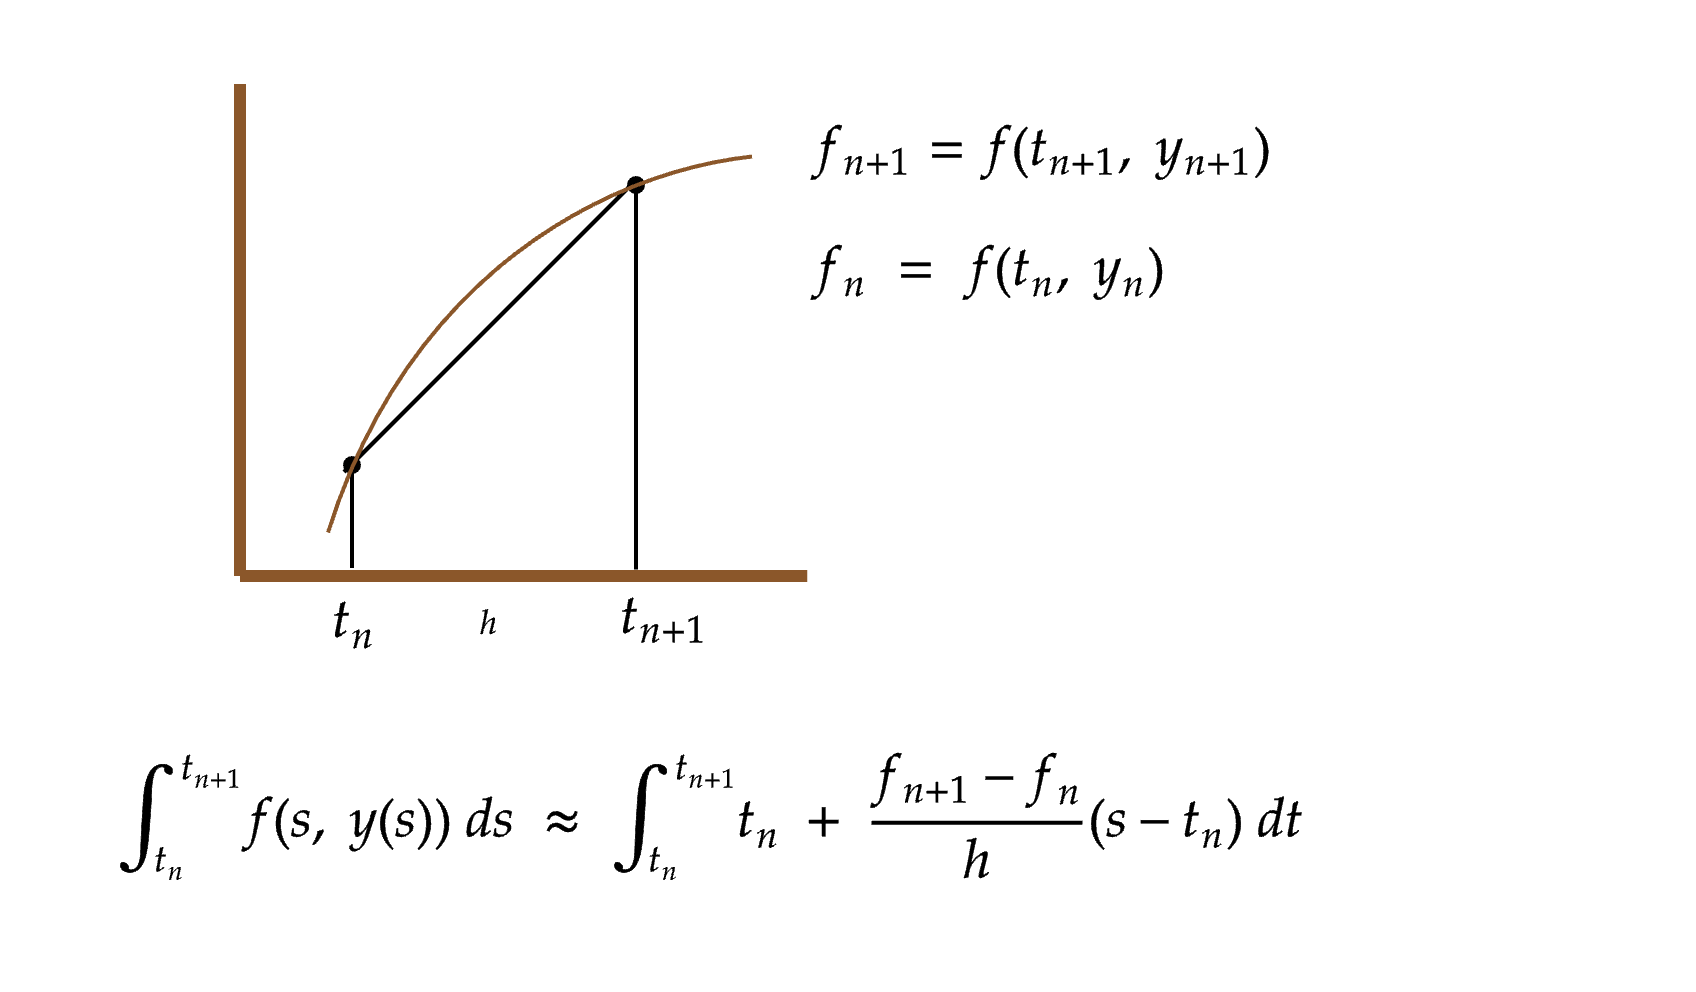
\includegraphics[width=0.8\textwidth]{figures/fig-24.png}
\end{center}

\begin{defn}[Trapezoidal Method]
	The \textbf{trapezoidal method} is,
	\[y_{n+1} = y_n + \frac{h}{2} \cdot (f_{n+1} + f_n)\]
	which is $1$-step implicit.
\end{defn}

\noindent We will see two alternatives to this method,

\begin{defn}[Adam-Bashford]
	The \textbf{Adam-Bashford} method is,
	\[y_{n+1} = y_n + \frac{h}{2} \cdot (3f_n - f_{n-1})\]
	which is $2$ step explicit.
\end{defn}

\begin{defn}[Adam-Moulton]
	The \textbf{Adam-Moulton} method is,
	\[y_{n+1} = y_n + \frac{h}{12} \cdot (5 f_{n+1} + 8 f_n - f_{n-1})\]
	which is $2$ step implicit.
\end{defn}

\begin{ex}{Newton's Law of Cooling}{label}
	Given a constant $k > 0$, the change in temperature $T(t)$ of an object due to conduction is as follows,
	\[
	\begin{cases}
		T^{\prime}(0) = -k(T(t) - T_{\texttt{env}}) & \\
		T(0) = T_0
	\end{cases}
	\]
	where $T_{\texttt{env}}$ is the environment temperature, and $T_0$ is the initial temperature. The exact solution is,
	\[T(t) = (T_0 - T_{\texttt{env}})e^{-kt} + T_{\texttt{env}}\]
	We can use the three $1$-step methods to solve our system,
	\begin{enumerate}
	\item Forward Euler's Method gives,
	\[T_{n+1}=T_n+h\left(-k\left(T_n-T_{\texttt{env}}\right)\right)\]
	\item Backward Euler's Method gives,
	\[T_{n+1}=T_n+h\left(-k\left(T_{n+1}-T_{\texttt{env}}\right)\right)\]
	\item The Trapezoidal Method gives,
	\[T_{n+1}=T_n+\frac{h}{2}\left(-k\left(T_{n+1}-T_{\texttt{env}}\right)-k\left(T_n-T_{\texttt{env}}\right)\right)\]
	\end{enumerate}
	To compare the accuracy of each method, we look at the error
	\[|T_N(1) - T(1)|\]
	$N$ increases, equivalently, as $h$ decreases.
	\[
	\begin{array}{|c|c|c|c|}
	\hline h & \text {Forward} & \text {Backward} & \text{Trapezoidal} \\
	\hline \hline 0.05 & 1.0318971 & 0.9981259 & 0.0169282 \\
	0.025 & 0.5117345 & 0.5032799 & 0.0042299 \\
	0.0125 & 0.2548108 & 0.2526965 & 0.0010574 \\
	0.00625 & 0.1271411 & 0.1266125 & 0.0002643 \\
	\hline
	\end{array}
	\]
	We can estimate the order $\mathcal{O}\left(h^p\right)$ of each method using the slope of the log-log plot in the error versus $h$. We get that,
	\begin{enumerate}
		\item Forward and Backward Euler have a slope of $1$, i.e., $\mathcal{O}(h)$
		\item The Trapezoidal Method has a slope of $2$, i.e., $\mathcal{O}(h^2)$
	\end{enumerate}
\end{ex}

\begin{marginfigure}
	\begin{center}
       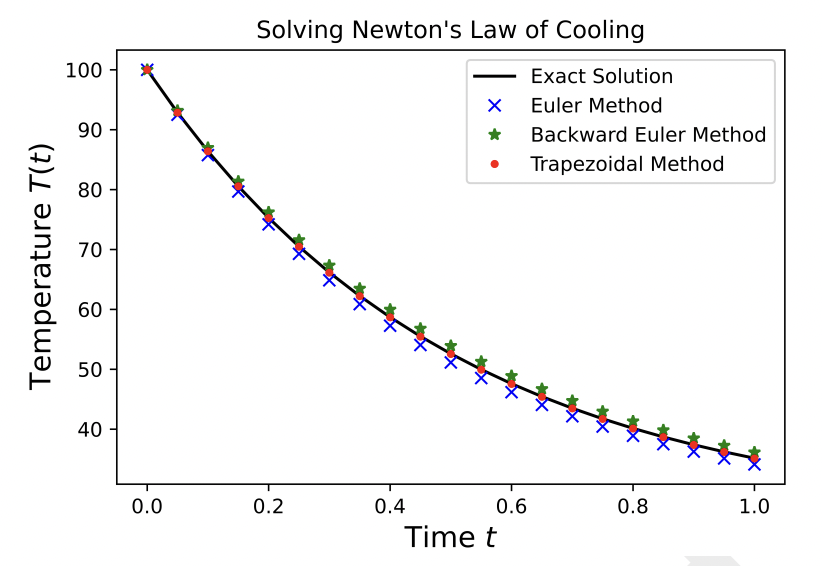
\includegraphics[width=\textwidth]{figures/fig-25.png}
       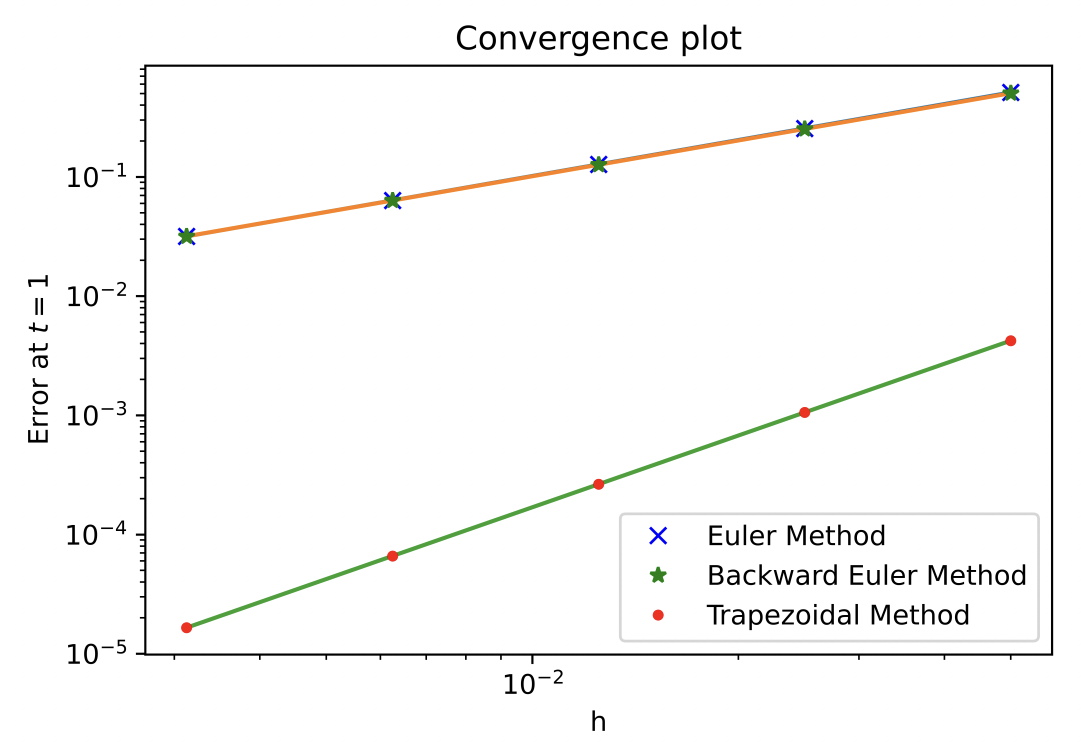
\includegraphics[width=\textwidth]{figures/fig-26.png}
	\end{center}
\end{marginfigure}

\subsection{Error Analysis}
We want to \textbf{quantify the error} in approximating initial value problems as the step size approaches $0$. To do this, we will re-write our $k$-step discretization scheme as the zero of a map $\phi$,
\[\phi_h(t_n, y_{n+1}, y_n, \cdots, y_{n-k+1}) = 0\]
which is satisfied for the unknown $y_{n+1}$.

\begin{defn}[Local Truncation Error]
	The \textbf{local truncation error} is,
	\[\tau_h\left(t_n\right):=\Phi_h\left(t_n, y\left(t_{n+1}\right), y\left(t_n\right), \ldots, y\left(t_{n-k+1}\right)\right)\]
\end{defn}

\begin{rmk}
In general, $\tau_h\left(t_n\right)=\mathcal{O}\left(h^p\right)$ for some power $p$.
\end{rmk}

\begin{ex}{Local Truncation Error for Euler's Method}{label}
	We will bound the local truncation error for Euler's method. Let $y$ be a solution to the initial value problem. Then,
	\begin{align*}
	\tau_h\left(t_n\right) &:=\Phi_h\left(t_n, y\left(t_{n+1}\right), y\left(t_n\right)\right) \\
	&=y\left(t_{n+1}\right)-y\left(t_n\right)-h f\left(t_n, y\left(t_n\right)\right) \\
	&=\left(y\left(t_n\right)+y^{\prime}\left(t_n\right) h+\frac{y^{\prime \prime}\left(\xi_n\right)}{2} h^2\right)-y\left(t_n\right)-h f\left(t_n, y\left(t_n\right)\right) \\
	&=h \underbrace{\left(y^{\prime}\left(t_n\right)-f\left(t_n, y\left(t_n\right)\right)\right.}_{= 0}+\frac{y^{\prime \prime}\left(\xi_n\right)}{2} h^2
	\end{align*}
	for $\xi_n \in (t_n, t_{n+1})$ obtained by  Taylor's Theorem. Define,
	\[M_2:=\max _{t \in[0, T]}\left|y^{\prime \prime}(t)\right|\]
	It follows that,
	\[\left|\tau_h\left(t_n\right)\right| \leq \frac{M_2}{2} h^2\]
	and therefore $\tau_h\left(t_n\right)=\mathcal{O}\left(h^2\right)$.
\end{ex}

\begin{defn}[Global Truncation Error]
	The \textbf{global truncation error} is,
	\[\frac{\tau_h}{h}=\frac{1}{h} \cdot \max _{0 \leq n \leq N} |\tau_h\left(t_n\right)|\]
\end{defn}

\begin{rmk}
	A method is of order $p$ if,
	\[\frac{\tau_h}{h}=\mathcal{O}\left(h^p\right)\]
	This condition holds if and only if $\tau_h\left(t_n\right)=\mathcal{O}\left(h^{p+1}\right)$.
\end{rmk}

\begin{defn}[Consistency]
	A method is \textbf{consistent} if,
	\[\lim _{h \rightarrow 0} \frac{\tau_h}{h}=0\]
\end{defn}

\begin{rmk}
	If a method is of order \text{$p > 0$}, then it is consistent.
\end{rmk}

\begin{ex}{Consistency of Euler's Method}{label}
	We determined in the previous example that,
	\[\left|\tau_h\left(t_n\right)\right| \leq C h^2\]
	for some $C > 0$ independent of $t_n$. Thus,
	\[\frac{\tau_h}{h}=\max _{0 \leq n \leq N} \frac{\left|\tau_h\left(t_n\right)\right|}{h}=\mathcal{O}(h)\]
	so Euler's method is of order $1$ and hence consistent.
\end{ex}

\begin{defn}[Convergence]
	A method is called \textbf{convergent} if,
	\[\lim _{h \rightarrow 0} \max _{0 \leq n \leq N}|\underbrace{y(t_n) - y_n}_{e_n}|=0\]
	where $e_n$ denotes the error at time $t_n$.
\end{defn}

\begin{thm}[Convergence of Euler's Method]
	Let $f: [0, T] \times \R \rightarrow \R$ be continuous in $t$ and continuously differentiable in $y$. If there exists $L > 0$ such that
	\[\left|\frac{\partial f}{\partial z}(t, y)\right| \leq L \forall (t, y) \in [0, T] \times \R\]
	then the Euler method converges.
\end{thm}

\begin{proof}
	By definition of Euler's method,
	\[(\star) \quad y_{n+1}=y_n+h f\left(t_n, y_n\right)\]
	and the local trunction error is,
	\[\tau_h\left(t_n\right)=y\left(t_{n+1}\right)-y\left(t_n\right)-h f\left(t_n, y\left(t_n\right)\right)\]
	Re-arranging for $y(t_{n+1})$ gives that,
	\[y\left(t_{n+1}\right)=y\left(t_n\right)+h f\left(t_n, y\left(t_n\right)\right)+\tau_h\left(t_n\right)\]
	Subtracting by $(\star)$ gives that,
	\[e_{n+1}=e_n+h\left(f\left(t_n, y\left(t_n\right)\right)-f\left(t_n, y_n\right)\right)+\tau_h\left(t_n\right)\]
	By the Mean Value Theorem, $\exists \xi_n \in (y(t_n), t_n)$ such that,
	\[f\left(t_n, y\left(t_n\right)\right)-f\left(t_n, y_n\right) = \frac{\partial f}{\partial z}\left(t_n, \xi_n\right)\left(y\left(t_n\right)-y_n\right)\]
	The following inequalities hold by assumption and by definition,
	\[\left|\frac{\partial f}{\partial z}(t, z)\right| \leq L \quad \quad \left|\tau_h\left(t_h\right)\right| \leq \tau_h\]
	It follows that,
	\begin{align*}
	\left|e_{n+1}\right| & \leq\left|e_n\right|+h L\left|e_n\right|+\tau_h \\
	&=(1+h L)\left|e_n\right|+\tau_h \\
	& \leq(1+h L)\left((1+h L)\left|e_{n-1}\right|+\tau_h\right)+\tau_h \\
	&=(1+h L)^2\left|e_{n-1}\right|+(1+(1+h L)) \tau_h \\
	& \leq \ldots
	\end{align*}
	Repeating inductively,
	\[\left|e_{n+1}\right| \leq(1+h L)^{n+1}\left|e_0\right|+\left(1+(1+h L)+\ldots+(1+h L)^n\right) \tau_h\]
	where $|e_0| = 0$. Summing the geometric series,
	\[\sum_{i=0}^n(1+h L)^i = \frac{(1+h L)^{n+1}-1}{(1+h L)-1}\]
	so that our bound can be simplified as follows,
	\begin{align*}
	|e_{n+1}|
	&\leq \frac{(1+h L)^{n+1}-1}{h L} \tau_h \\
	&\leq \frac{e^{(n+1) h L}-1}{L} \frac{\tau_h}{h} \quad \text{ since } 1 + x \leq e^x \text{ for all } x \in \R \\
	&\leq \frac{e^{N h L}-1}{L} \frac{\tau_h}{h} \quad \text{ since } 0 \leq n + 1 \leq N
	\end{align*}
	Using the fact that $T = n \cdot h$, 
	\[\left|e_{n+1}\right| \leq \underbrace{\frac{e^{T L}-1}{L}}_{C} \cdot \frac{\tau_h}{h}\]
	It follows that Euler's method is consistent since $C$ is a constant that does not depend on $h$. That is, as $h \rightarrow 0$,
	\[\left|e_{n+1}\right| \leq C \frac{\tau_h}{h} \rightarrow 0\]
\end{proof}

\NewLine

\noindent While all $1$ step methods are convergent, we will see that not every consistent $k$-step method converges. We require some additional notion of \textbf{stability} to guarantee convergence for $k \geq 2$ step methods.

\begin{defn}[Linear Multistep Method]
	A $k$-step method is a \textbf{linear multistep method} if the discretization can be written as
	\[y_{n+1}+\sum_{i=0}^{k-1} a_{k-1-i} y_{n-i}=h\left(b_k f_{n+1}+\sum_{i=0}^{k-1} b_{k-1-i} f_{n-i}\right)\]
	where $a_i$ and $b_i$ are constants and $f_i = f(t_i, y_i)$. Equivalently, 
	\[\Phi_h:=y_{n+1}+\sum_{i=0}^{k-1} a_{k-1-i} y_{n-i}-h\left(b_k f_{n+1}+\sum_{i=0}^{k-1} b_{k-1-i} f_{n-i}\right)=0\]
\end{defn}

\begin{rmk}
	The discretization $\Phi_h$ of a $k$-step linear multistep method is linear in $y_{n+1}, \ldots, y_{n-k+1}$ and $f_{n+1}, \ldots, f_{n-k+1}$.
\end{rmk}

\begin{rmk}
	If $b_k = 0$, then the method is explicit. Otherwise,
	\[y_{n+1}+\sum_{i=0}^{k-1} a_{k-1-i} y_{n-i}=h\left(\sum_{i=0}^{k-1} b_{k-1-i} f_{n-i}\right)\]
	and the method is implicit.
\end{rmk}

\begin{ex}{Central Difference Method}{label}
	Pick $a_0 = -1$, $a_1 = 0$, $b_0 = 0$, $b_1 = 2$, and $b_2 = 0$. This gives,
	\[y_{n+1}=y_{n-1}+2 h f_n\]
\end{ex}

\begin{ex}{Adam-Bashford Method}{label}
	Pick $a_0=0, a_1=-1, b_0=-\frac{1}{2}, b_1=\frac{3}{2}$ and $b_2=0$. This gives,
	\[y_{n+1}=y_n+\frac{h}{2}\left(3 f_n-f_{n-1}\right)\]
\end{ex}

\begin{ex}{Adam-Moulton Method}{label}
	Pick $a_0=0, a_1=-1, b_0=-\frac{1}{12}, b_1=\frac{2}{3}$ and $b_2=\frac{5}{12}$. This gives,
	\[y_{n+1}=y_n+\frac{h}{12}\left(5 f_{n+1}+8 f_n-f_{n-1}\right)\]
\end{ex}

\NewLine

\noindent Using Taylor's Theorem, we can derive a set of \textbf{order} and \textbf{consistency} conditions for $k$-step linear multistep methods. These are:

\begin{thm}[Consistency Conditions]
	A $k$-step linear multistep method is \textbf{consistent} if and only if we have:
	\begin{align*}
	&\sum_{i=0}^{k-1} a_i=-1 \\
	&\sum_{i=0}^k b_i=k+\sum_{i=0}^{k-1} i \cdot a_i
	\end{align*}
\end{thm}

\begin{thm}[Order Conditions]
	A $k$-step linear multistep method is of \textbf{order} $p$ if and only for $q = 1, \ldots, p$ we have:
	\begin{align*}
		&\sum_{i=0}^{k-1} a_i=-1 \\
		&q \sum_{i=0}^k i^{q-1} \cdot b_i=k^q+\sum_{i=0}^{k-1} i^q \cdot a_i \\
	\end{align*}
	
\end{thm}

\begin{marginfigure}
	Not all consistent linear multistep methods are convergent.
\end{marginfigure}

\begin{ex}{Consistent but Divergent Linear Multistep Methods}{label}
	Consider the following $2$ step explicit linear multistep method,
	\[y_{n+1}+4 y_n-5 y_{n-1}=h\left(4 f_n+2 f_{n-1}\right)\]
	The constants $a_i$ and $b_i$ are determined as follows,
	\[a_1=4, a_0=-5 \text { and } b_2=0, b_1=4, b_0=2\]
	This method is of order $3$ by the order conditions and hence it is consistent. We will apply it to the IVP
	\[\left\{\begin{array}{l}
	y^{\prime}(t)=-y(t) \\
	y(0)=1
	\end{array}\right.\]
	which we know has the following solution
	\[y(t) = e^{-t}\]
	for all $t \geq 0$. Using Euler's method to initialize $y_1$, we obtain an error that tends to infinity as $h \rightarrow 0$. This is shown below,
	\[\begin{array}{|c|c|}
	\hline h & \left|y(1)-y_N\right| \\
	\hline \hline 0.2 & 11.7 \\
	\hline 0.1 & 6.51 \times 10^3 \\
	\hline 0.05 & 2.37 \times 10^8 \\
	\hline
	\end{array}\]
	Therefore, consistency is insufficient for convergence.
\end{ex}

\NewLine

The previous example motivates the need for aa stronger condition that consistency to guarantee convergence. We require some idea of the stability of the system, which we will formalize using the concept of \textbf{zero-stability}. We begin with basic definitions.

\NewLine

\begin{defn}[Characteristic Polynomial]
	Let $\{a_i\}$ be the coefficients of a linear multistep method. The \textbf{characteristic polynomial} is,
	\[p(\lambda)=\lambda^k+a_{k-1} \lambda^{k-1}+\ldots a_1 \lambda+a_0\]
\end{defn}

\begin{defn}[Zero-Stability]
	Let $\{\lambda_1, \cdots, \lambda_k\}$ be the roots of the characteristic polynomial. The conditions for \textbf{zero-stability} are,
	\begin{enumerate}
		\item $|\lambda_i| \leq 1$
		\item $|\lambda_i| = 1 \implies \lambda_i \neq \lambda_j$ for all $j \neq i$
	\end{enumerate}
	That is, all roots have modulus less than or equal to $1$ and all roots of modulus equal to $1$ are distinct.
\end{defn}

\begin{ex}{Central Difference Method}{label}
	Since $a_0 = -1$ and $a_1 = 0$,
	\[p(\lambda)=\lambda^2-1=(\lambda-1)(\lambda+1)\]
	and zero-stability holds.
\end{ex}

\begin{ex}{Divergent Method}{label}
	Since $a_0 = -5$ and $a_1 = 4$,
	\[p(\lambda)=\lambda^2+4\lambda-5=(\lambda+5)(\lambda-1)\]
	and zero-stability does not hold.
\end{ex}

\begin{thm}[Convergence of Linear Multistep Methods]
	Consistent linear multistep methods converge $\iff$ zero-stability holds.
\end{thm}

\begin{cor}
	If a consistent linear multistep method converges, then it converges at the same order as the consistency error.
\end{cor}

\begin{marginfigure}
	In summary,
	\begin{enumerate}
		\item Consistency implies convergence for $1$ step methods
		\item Consistency and the order conditions imply convergence for linear multistep methods
		\item Consistent linear multistep methods converge if and only if zero-stability holds
	\end{enumerate}
\end{marginfigure}

\begin{ex}{Adam-Bashford}{label}
	We want to find the order of the Adam-Bashford method and show that it converges. This method is $2$ step explicit,
	\[y_{n+1}=y_n+\frac{h}{2}\left(3 f_n-f_{n-1}\right)\]
	Re-arranging gives,
	\[y_{n+1}-y_n=\frac{h}{2}\left(3 f_n-f_{n-1}\right)\]
	and hence the coefficients are $a_0 = 0$, $a_1 = -1$, $b_0 = -\frac{1}{2}$, $b_1 = \frac{3}{2}$, and $b_2 = 0$. The characteristic polynomial is,
	\[p(\lambda)=\lambda^2-\lambda+0=\lambda(\lambda-1)\]
	which implies zero-stability. By the convergence theorem for linear multistep methods, it is sufficient so prove consistency. While this can be done using the conditions, we will prove it directly from the definitions. Since,
	\[\Phi_h=y_{n+1}-y_n-\frac{h}{2}\left(3 f_n-f_{n-1}\right)=0\]
	the local truncation error $\tau_h\left(t_n\right)$ is,
	\[=y\left(t_{n+1}\right)-y\left(t_n\right)-\frac{h}{2} \left(3 \underbrace{f\left(t_n, y\left(t_n\right)\right)}_{=y^{\prime}\left(t_n\right)}-\underbrace{f\left(t_{n-1}, y\left(t_{n-1}\right)\right)}_{=y^{\prime}\left(t_{n-1}\right)}\right)\]
	where $y(t)$ is the exact solution to the IVP. Applying Taylor's Theorem to $y$ and $y^{\prime}$ around $t_n$ gives that,
	\begin{align*}
		&y\left(t_{n+1}\right)=y\left(t_n\right)+y^{\prime}\left(t_n\right) h+\frac{y^{\prime \prime}\left(t_n\right)}{2} h^2+\frac{y^{(3)}\left(\xi_n\right)}{3 !} h^3 \\
		&y^{\prime}\left(t_{n-1}\right)=y^{\prime}\left(t_n\right)-y^{\prime \prime}\left(t_n\right) h+\frac{y^{(3)}\left(\eta_n\right)}{2} h^2
	\end{align*}
	for $\xi_n \in (t_n, t_{n+1})$ and $\nu_n \in (t_{n-1}, t_n)$. Thus,
	\[\tau_h(t_n)=\frac{1}{12}\left(2 y^{(3)}\left(\xi_n\right)+3 y^{(3)}\left(\eta_n\right)\right) h^3\]
	Define a constant $M_3=\max _{t \in[0, T]}\left|y^{(3)}(t)\right|$ so that,
	\[\left|\tau_h\left(t_n\right)\right| \leq \frac{5 M_3}{12} h^3\]
	The consistency error is,
	\[\frac{\tau_h}{h}=\max _{0 \leq n \leq N} \frac{\left|\tau_h\left(t_n\right)\right|}{h} \leq \frac{5 M_3}{12} h^2=\mathcal{O}\left(h^2\right) \rightarrow 0 \text { as } h \rightarrow 0\]
	from which we conclude that Adam-Bashford is consistent of order $2$ and zero-stable. This is sufficient for convergence.
\end{ex}

\subsection{Case Study: $A$-Stability}
The zero-stability condition is useful in concluding that a consistent linear multi-step method converges in the limit as $h \rightarrow 0$. In practice, we want to work with a fixed non-zero $h$. For efficiency, we want to take $h$ to be as large as possible. However, there are restrictions on $h$ that arise based on the methods that is being used.

Consider the following problem. Fix $\lambda \in \C$ with $\text{Re}(\lambda) < 0$. 
\begin{align}
	&\left\{\begin{array}{l}
	y^{\prime}(t)=\lambda y(t) \\
	y(0)=y_0
	\end{array}\right.
\end{align}
has $y(t) = y_0 \cdot e^{\lambda t}$ as an exact solution. We call the problem \textbf{stiff} if $\text{Re}(\lambda) \ll 0$. Observe that $y \rightarrow 0$ as $t \rightarrow \infty$, but numerical solutions do not always have this property. We will apply $1$ step methods, beginning with Euler's method, to see why this is the case.

\NewLine

\begin{ex}{Applying Euler's Method to $(1)$}{label}
	Iterating the recurrence that we obtain by definition:
	\begin{align*}
		y_{n+1}&=y_n+h \lambda y_n \\
		&=(1+h \lambda) y_n \\
		&=(1+h \lambda)^2 y_{n-1} \\
		&\cdots \\
		&= (1+h \lambda)^{n+1} y_0
	\end{align*}
	We require that $|1 + h \lambda| < 1$ for $y_n \rightarrow 0$ as $n \rightarrow \infty$ when $h$ is fixed. This condition is equivalent to the condition that,
	\[(1+x)^2 + y^2 < 1\]
	where $\lambda h = x + iy$. Observe that,
	\[|1 + h \lambda| = |1 + x + iy| \leq |1 + x| + |iy| = (1+x)^2 + y^2\]
	This region forms a circle in $\R^2$,
	\begin{center}
       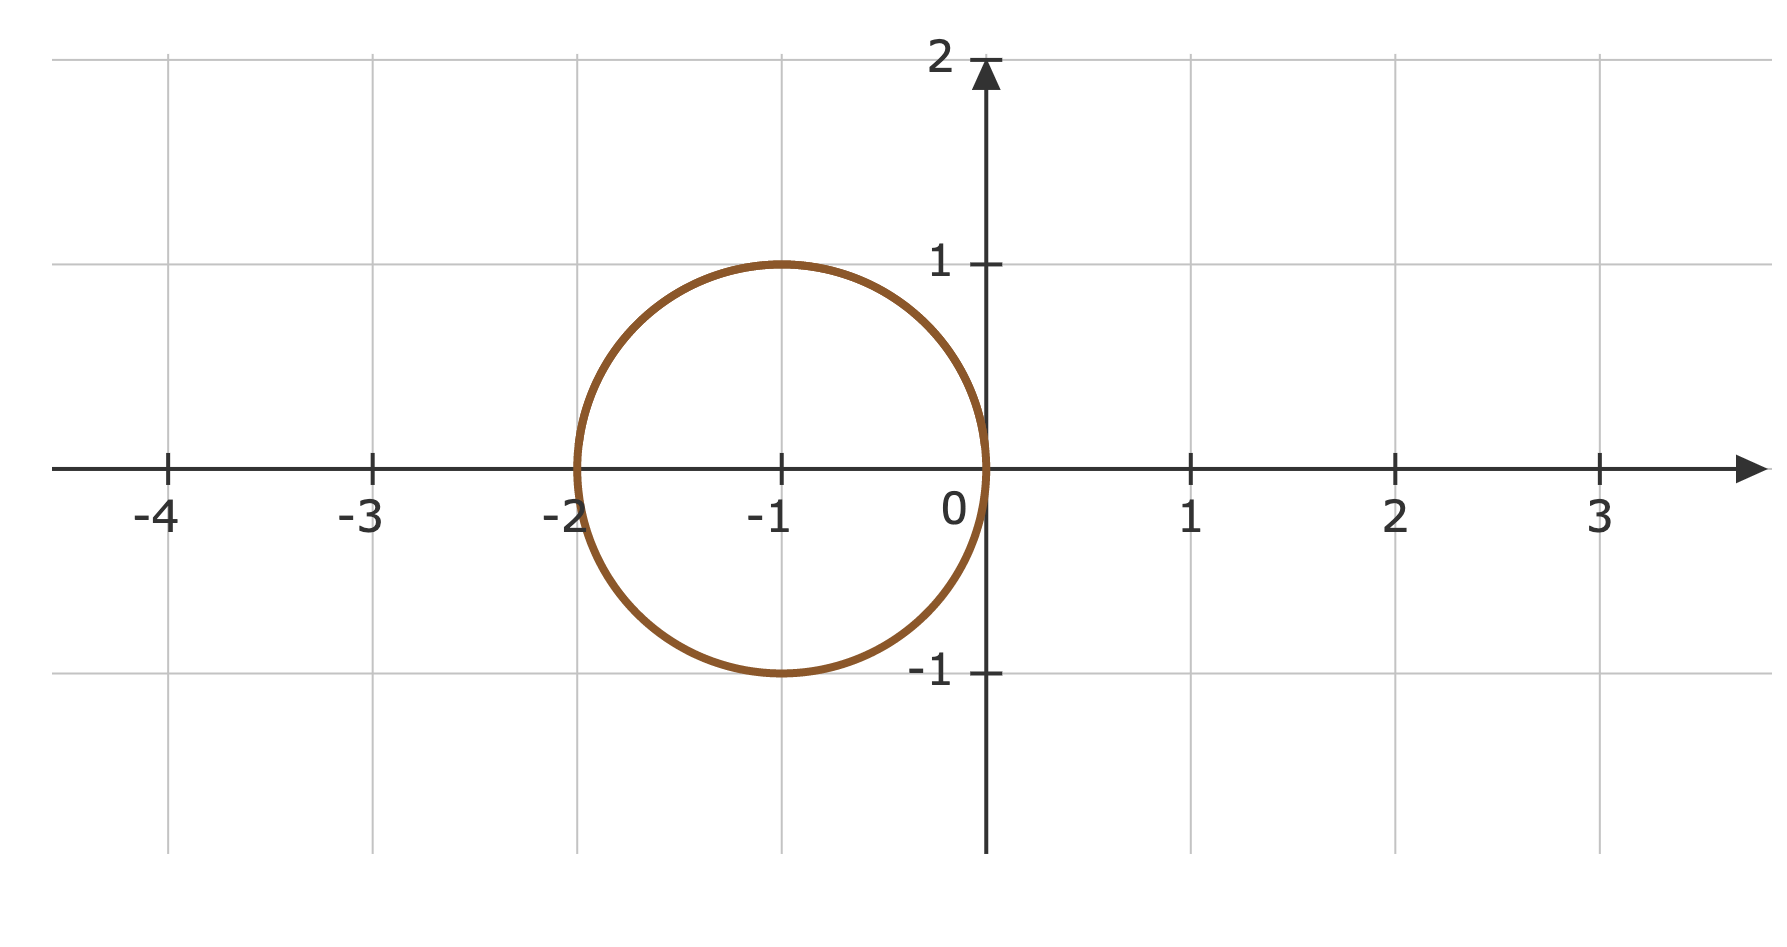
\includegraphics[width=0.8\textwidth]{figures/fig-27.png}
       \end{center}
       If $\lambda \in \R$, then we require
       \[|1+h\lambda| < 1 \iff -2 < h\lambda < 0 \iff 0 < h < -\frac{2}{\lambda}\]
       so the stiffer the problem, the smaller $h$ is required to be.

\end{ex}

\begin{ex}{Applying Backward Euler to $(1)$}{label}
	Iterating the recurrence that we obtain by definition:
	\begin{align*}
		y_{n+1} &= y_n + h\lambda y_{n+1} \\
			 &= \frac{y_n}{1-h\lambda} \\
			 &\cdots \\
			 &= \frac{y_0}{(1-\lambda h)^{n+1}}
	\end{align*}
	For fixed $h$, we require the same condition,
	\[|1-h\lambda| > 1 \iff (1-x)^2+y^2 > 1\]
	to have $y_n \rightarrow 0$ as $n \rightarrow \infty$. This region forms a circle in $\R^2$,
	\begin{center}
       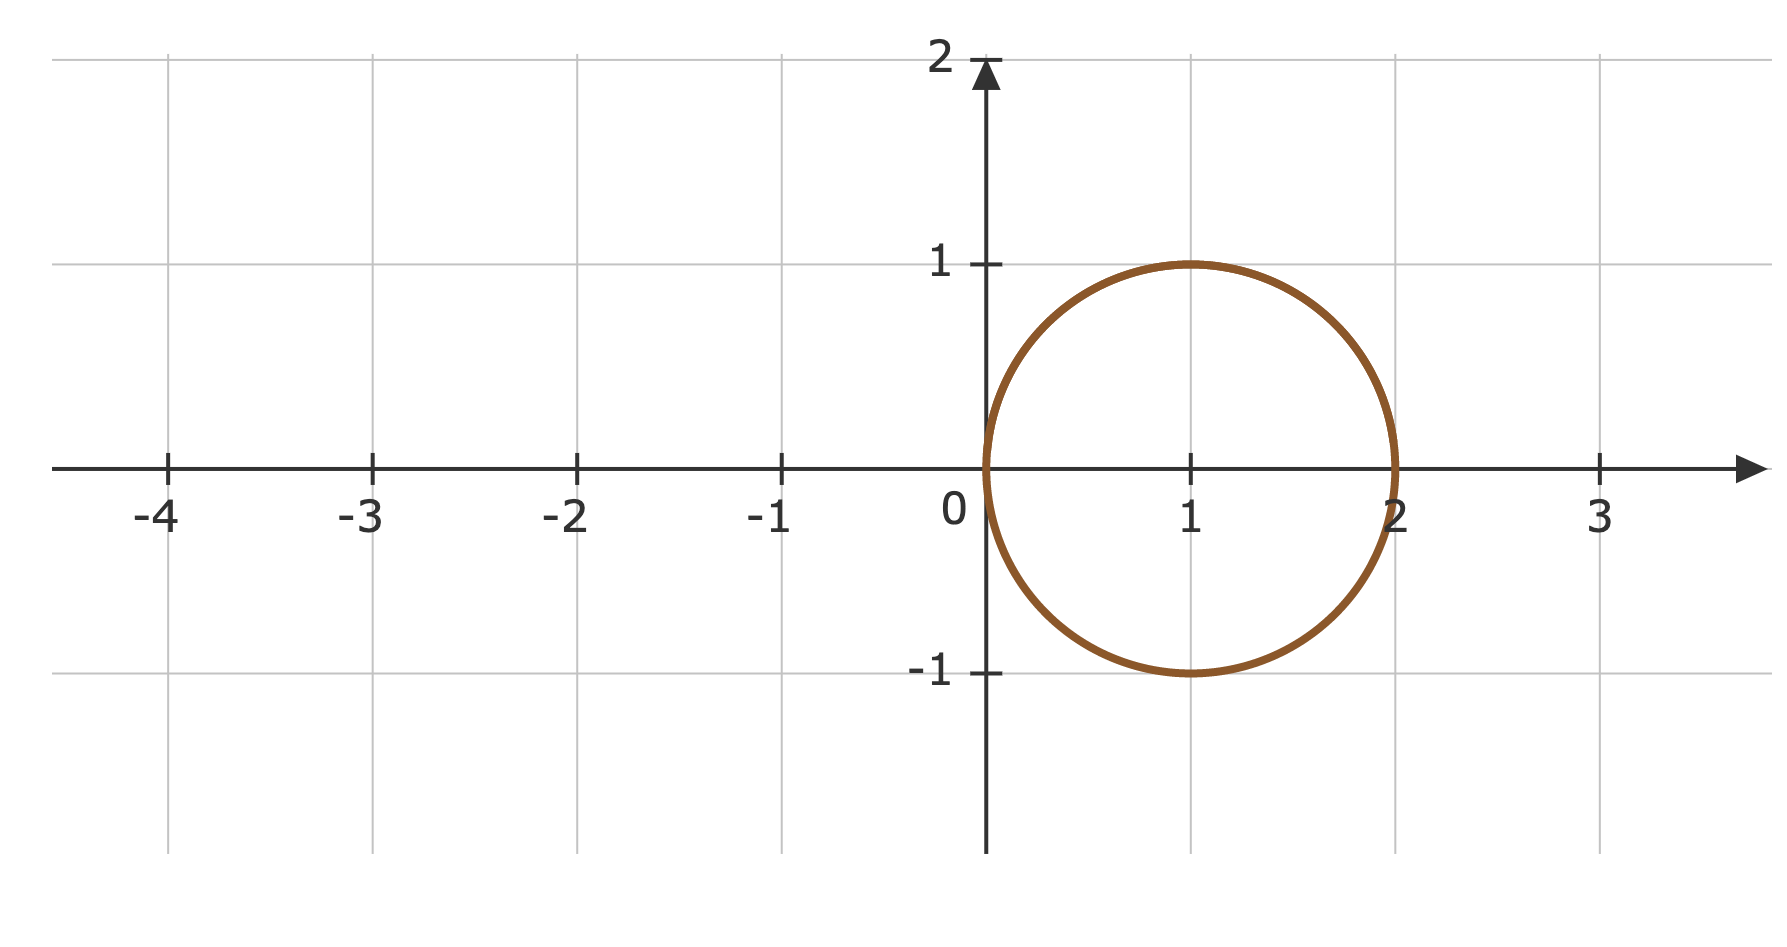
\includegraphics[width=0.8\textwidth]{figures/fig-28.png}
       \end{center}
       If $\lambda \in \R$, then we require
       \[|1-h\lambda| > 1 \iff h \lambda < 0 \text{ or } h \lambda > 2\]
       but $h \lambda < 0$ is satisfied since
       \[\text{Re}(\lambda) < 0\]
       so there is no restriction on $h$.
\end{ex}

\begin{ex}{Applying Trapezoidal to $(1)$}{label}
	We obtain by definition that,
	\[y_{n+1}=y_n+\frac{h}{2} \cdot\left(f_{n+1}+f_n\right)\]
	where $f\left(t_n, y_n\right)=\lambda \cdot y_n$. Re-arranging and iterating,
	\[y_{n+1}=\frac{y_n\left(1+\frac{h}{2} \lambda\right)^{n+1}}{\left(1-\frac{h}{2} \lambda\right)}\]
	If $h \lambda$ satisfies the inequality,
	\[1+\frac{h \lambda}{2} < 1 - \frac{h\lambda}{2}\]
	that is $h < 0$
	then $y_n \rightarrow 0$ as $n \rightarrow \infty$. If $\lambda \in \R$, then $\text{Re}(\lambda) < 0$ is satisfied. Hence, there is no restriction on the size of $h$.
\end{ex}

These examples on explicit and implicit $1$ step methods motivate the following definition of \textbf{$A$-stability} for problem $(1)$:

\begin{defn}[$A$-Stability]
	Let $h$ be fixed. If $y_n$ is the solution at $t_n$ of a method applied to $(1)$, then the region of \textbf{$A$-stability} is
	\[R=\left\{h \lambda \in \mathbb{C} \mid \lim _{n \rightarrow \infty} y_n \rightarrow 0, \text { for a fixed } h\right\} \subseteq \C\]
\end{defn}

\begin{rmk}
	An $A$-stable method is one with no restrictions on $h$.
\end{rmk}

\begin{ex}{$A$-Stability}{label}
	\begin{enumerate}
		\item Euler's method is not $A$-stable
		\item All explicit methods are not $A$-stable
		\item Backward Euler and the Trapezoidal method are $A$-stable
	\end{enumerate}
\end{ex}

\begin{marginfigure}
	For stiff problems, use an $A$-stable method or non-$A$ stable method with a large region $R$ in the left half of the complex plane.
\end{marginfigure}

\begin{marginfigure}
	Implicit methods tend to have larger regions of $A$-stability.
\end{marginfigure}

\NewLine

$A$-stability applies to equations other than $(1)$. We begin with definitions. Consider a one-dimensional autonomous system,
\begin{align}
	y^{\prime}(t) = f(y(t))
\end{align}
An \textbf{equilibrium solution} of $(2)$ is a solution $y^* \in \R$ such that $f(y^*) = 0$. We call $y^*$ \textbf{asymptotically stable} if $f^{\prime}(y^*) < 0$.
\[y^{\prime}=f(y)=\underbrace{f\left(y^*\right)}_{=0}+f^{\prime}\left(y^*\right)\left(y-y^*\right)+\frac{f^{\prime \prime}(\eta)}{2}\left(y-y^*\right)^2\]
for some $\eta$ guaranteed by Taylor's remainder theorem. For $\tilde{y}(t):=y(t)-y^*$, we can approximate the IVP as,
\[\tilde{y}^{\prime} \approx f^{\prime}\left(y^*\right) \tilde{y}\]
which is the same form as $(1)$ with $\lambda = f^{\prime}(y^*)$. This last step can be justified by the \textbf{linearization theorem} from dynamical systems.

\begin{rmk}
	If $y^*$ is asymptotically stable equilibrium, then $A$-stable methods will compute the correct $y^*$ without restrictions to $h$. In contrast, a method which is not $A$-stable can lead to unbounded growh or oscillations near $Y^*$ if $h$ is not small enough. 
\end{rmk}

\begin{ex}{$A$-Stability}{label}
	Suppose that a method is $A$-stable. We may be tempted to take $h$ large enough to compute $y(T)$ with one time step.
	\begin{enumerate}
		\item The error is still $\mathcal{O}(h^p)$
		\item Since all $A$-stable methods are implicit, root finding methods may not converge if $h$ is too large
	\end{enumerate}
\end{ex}

\subsection{Predictor-Corrector Methods}
While implicit methods have notable stability properites, one main drawback is the requirement that we use root finding methods. In this section, we will explore \textbf{predictor-corrector} as a potential solution to this. The basic idea will be to use an explicit method to predict $y_{n+1}$, prior to correct $y_{n+1}$ using the implicit method.

\begin{defn}[Improved Euler Method]
	The \textbf{I-Euler method} is,
	\[y_{n+1}=y_n+\frac{h}{2}\left(f\left(t_n, y_n\right)+f\left(t_{n+1}, \tilde{y}_{n+1}\right)\right)\]
	which is obtained by using the Euler method to predict $y_{n+1}$,
	\[\begin{array}{ll}
	\tilde{y}_{n+1}=y_n+h f\left(t_n, y_n\right) & \text { (predict) } \\
	&\\
	y_{n+1}=y_n+\frac{h}{2}\left(f\left(t_n, y_n\right)+f\left(t_{n+1}, \tilde{y}_{n+1}\right)\right) & \text { (correct) }
	\end{array}\]
	in the original trapezoidal method,
	\[y_{n+1}=y_n+\frac{h}{2}\left(f\left(t_n, y_n\right)+f\left(t_{n+1}, y_{n+1}\right)\right)\]
	Substituting $\tilde{y}_{n+1}$,
	\[y_{n+1}=y_n+\frac{h}{2}\left(f\left(t_n, y_n\right)+f\left(t_{n+1}, y_n+h f\left(t_n, y_n\right)\right)\right)\] 
\end{defn}

\noindent This is a $1$ step method, so it suffices to show consistency in order to show convergence. It is not multistep, so we cannot use the order conditions. We will compute the consistency error.
\[\Phi_h=y_{n+1}-y_n-\frac{h}{2}\left(f\left(t_n, y_n\right)+f\left(t_{n+1}, y_n+h f\left(t_n, y_n\right)\right)\right)\]
Let $y$ be the exact solution to the IVP. So the local truncation error is,
\[y\left(t_{n+1}\right)-y\left(t_n\right)-\frac{h}{2}\left(f\left(t_n, y\left(t_n\right)\right)+f\left(t_{n+1}, y\left(t_n\right)+h f\left(t_n, y\left(t_n\right)\right)\right)\right)\]
which we can simplify as follows,
\begin{align*}
	y^{\prime}\left(t_n\right) h &+\frac{y^{\prime \prime}\left(t_n\right)}{2} h^2+\mathcal{O}\left(h^3\right) \\
	&- \frac{h}{2}\left(f\left(t_n, y\left(t_n\right)\right)+f\left(t_{n+1}, y\left(t_n\right)+h f\left(t_n, y\left(t_n\right)\right)\right)\right)
\end{align*}

Since $y^{\prime}=f(t, y)$, differentiating in $t$ implies that,
\[y^{\prime \prime}=f_t(t, y)+f_y(t, y) y^{\prime}=f_t(t, y)+f_y(t, y) f(t, y)\]
Applying Taylor's Theorem to $f$ about the point $(t, y)$,
\[f(t+h, y+c h)=f(t, y)+f_t(t, y) h+f_y(t, y) c h+\mathcal{O}(h^2)\]
and setting $t = t_n$, $y = y(t_n)$, and $c = f(t_n, y(t_n))$ gives,
\[f\left(t_{n+1}, y\left(t_n\right)+h f\left(t_n, y\left(t_n\right)\right)\right)\]
which evaluates to,
\[f\left(t_n, y\left(t_n\right)\right)+f_t\left(t_n, y\left(t_n\right)\right) h+f_y\left(t_n, y\left(t_n\right)\right) f\left(t_n, y\left(t_n\right)\right) h+\mathcal{O}(h^2)\]
Simplifying $\tau_h\left(t_n\right)$ using this expression tells us that $\tau_h\left(t_n\right)=\mathcal{O}(h^3)$, therefore, $\tau_h=\mathcal{O}(h^2)$. Hence, the method is of order $2$.

\subsection{Runge-Kutta Methods}
Explicit $1$ step methods are fast and easy to implement, but they have low order accuracy. One idea is to generalize to higher order and take fractional time steps that allow us to compute $y_{n+1}$ in stages. This is the idea behind \textbf{Runge-Kutta (RK)} methods. The general form of an $s$-stage explicit RK method is,
\begin{align*}
k_1=& f\left(t_n+c_1 h, y_n\right) \\
k_2=& f\left(t_n+c_2 h, y_n+h a_{2,1} k_1\right) \\
k_3=& f\left(t_n+c_3 h, y_n+h\left(a_{3,1} k_1+a_{3,2} k_2\right)\right) \\
& \vdots \\
k_s=& f\left(t_n+c_s h, y_n+h\left(a_{s, 1} k_1+a_{s, 2} k_2+\cdots+a_{s, s-1} k_{s-1}\right)\right.\\
y_{n+1}=& y_n+h\left(b_1 k_1+\cdots+b_s k_s\right)
\end{align*}
The coefficients $b_i$ are called \textbf{weights}, $c_i$ are called \textbf{nodes}, $k_i$ are stages, and the entries $a_{i,j}$ form the \textbf{RK matrix}.

\begin{rmk}[Butcher Tableau]
	Runge-Kutta methods are specified by
	\[\begin{array}{c|c}
	\mathbf{c} & \mathbf{A} \\
	\hline & \mathbf{b}^{T}
	\end{array}\]
	where $\mathbf{c}$ is the column vector of nodes, $\mathbf{b}^T$ is the row vector of weights, and $A$ is the RK matrix.
\end{rmk}

\begin{cor}
	$A$ must be strictly lower triangular for the explicit RK method. Otherwise, the RK methods are implicit.
\end{cor}

\begin{ex}{Improved Euler as an RK Method}{label}
	I-Euler method can be written as a $2$ stage explicit RK method:
	\[
		\left\{\begin{aligned}
	k_1 &=f\left(t_n, y_n\right) \\
	k_2 &=f\left(t_n+h, y_n+h k_1\right), \\
	y_{n+1} &=y_n+h\left(\frac{1}{2} k_1+\frac{1}{2} k_2\right)
	\end{aligned}\right.
	\]
	Arranged in the RK Tableau, this becomes,
	\[\begin{array}{c|c}
	0 &  \\
	1 &  1 \\
	\hline & 1/2 \quad 1/2
	\end{array}\]
\end{ex}

\begin{ex}{$4$ Stage Explicit Runge-Kutta Method}{label}
	The most popular Runge-Kutta method is the following,
	\begin{align*}
	k_1 &=f\left(t_n, y_n\right) \\
	k_2 &=f\left(t_n+\frac{h}{2}, y_n+\frac{h}{2} k_1\right) \\
	k_3 &=f\left(t_n+\frac{h}{2}, y_n+\frac{h}{2} k_2\right) \\
	k_4 &=f\left(t_n+h, y_n+h k_3\right) \\
	y_{n+1} &=y_n+h\left(\frac{1}{6} k_1+\frac{1}{3} k_2+\frac{1}{3} k_3+\frac{1}{6} k_4\right)
	\end{align*}
	Arranged in the RK Tableau, this becomes,
	\[\begin{array}{c|cccc}
	0 & & & \\
	1/2 &  1 & & \\
	1/2 & 0 & 1/2 & \\
	1 & 0 & 0 & 1 \\
	\hline
	& 1/6 & 1/3 & 1/3 & 1/6
	\end{array}\]
	It can be shown that this method is of order $4$.
\end{ex}

\begin{marginfigure}
	RK$4$ is not $A$-stable, but both RK$4$ and I-Euler have larger regions of $A$-stability than previous explicit method, e.g., Euler and Adam-Bashford.
\end{marginfigure}

\subsection{First-Order Systems of ODEs}
We can generalize methods for solving first-order initial value problems to systems. Consider the system of first-order ODEs,
\[\left\{\begin{array}{l}
\mathbf{y}^{\prime}(t)=\mathbf{f}(t, \mathbf{y}(t)) \\
\mathbf{y}(0)=\mathbf{y}_0
\end{array}\right.\]
Euler's method can be written as,
\[\mathbf{y}_{n+1}=\mathbf{y}_n+h \mathbf{f}\left(t_n, \mathbf{y}_n\right)\]
and the Backward Euler method can be written as,
\[\mathbf{y}_{n+1}=\mathbf{y}_n+h \mathbf{f}\left(t_n, \mathbf{y}_{n+1}\right)\]
For implicit methods, root finding methods are required to solve the system. These include fixed point iteration and Newton's method. Linear multistep methods can also be applied to first order systems, where consistency and zero-stability results will hold. For example, $A$-stability can be applied to an autonomous system,
\[y^{\prime}=f(y)\]
where near an equilibrium solution $\mathbf{y}^*$,
\[\mathbf{y}^{\prime} \approx J_F\left(\mathbf{y}^*\right)\left(\mathbf{y}-\mathbf{y}^*\right)\]
Since the Jacobian $J_F\left(\mathbf{y}^*\right)$ is a matrix, the stiffness of the system will be determined by the eigenvalues of $J_F\left(\mathbf{y}^*\right)$ with negative real components. Predictor-corrector and Runge-Kutta methods also generalize. For instance, the I-Euler method can be generalized as,
\[\left\{\begin{aligned}
\mathbf{k}_1 &=\mathbf{f}\left(t_n, \mathbf{y}_n\right) \\
\mathbf{k}_2 &=\mathbf{f}\left(t_n+h, \mathbf{y}_n+h \mathbf{k}_1\right) \\
\mathbf{y}_{n+1} &=\mathbf{y}_n+h\left(\frac{1}{2} \mathbf{k}_1+\frac{1}{2} \mathbf{k}_2\right)
\end{aligned}\right.\]
The next example will show how we can write a higher-order IVP as a first-order system by introducing the appropriate variables.

\NewLine 

\begin{ex}{Solving Higher-Order IVPs}{label}
	Consider the second-order IVP,
	\[\left\{\begin{aligned}
	x^{\prime \prime}(t) &=f\left(t, x(t), x^{\prime}(t)\right) \\
	x(0) &=a \\
	x^{\prime}(0) &=b
	\end{aligned}\right.\]
	Define the following variables,
	\begin{align*}
		&y:=x^{\prime} \\
		&x^{\prime \prime}=f\left(t, x, x^{\prime}\right) \iff y^{\prime}=f(t, x, y)
	\end{align*}

	 Hence, the second-order IVP can be written as,
	\begin{align*} \mathbf{x}^{\prime}(t) &:=\left(\begin{array}{l}x^{\prime}(t) \\ y^{\prime}(t)\end{array}\right)=\left(\begin{array}{c}y(t) \\ f(t, x(t), y(t))\end{array}\right)=: \mathbf{f}(t, \mathbf{x}(t)) \\ \mathbf{x}(0) &:=\left(\begin{array}{c}x(0) \\ y(0)\end{array}\right)=\left(\begin{array}{l}a \\ b\end{array}\right)=: \mathbf{x}_0 \end{align*}
\end{ex}